%%%%%%%%%%%%%%%%%%%%%%%%%%%%%%%%%%%%%%%%%%%%%%%%%%%%%%%%%%%%%%%%%%%
%                                                                 %
%   HBOOK User Guide -- LaTeX Source                              %
%                                                                 %
%   Chapter 3                                                     %
%                                                                 %
%   The following external EPS files are referenced:              %
%                                                                 %
%   Editor: Michel Goossens / CN-AS                               %
%   Last Mod.:  9 Dec 1993 10:35 mg                               %
%                                                                 %
%%%%%%%%%%%%%%%%%%%%%%%%%%%%%%%%%%%%%%%%%%%%%%%%%%%%%%%%%%%%%%%%%%%
%  18.11.93: jds fix bugs in Ntuple examples
%  10.09.93: mg  add HFNOV
%

\index{Ntuple|(}
\index{RWN|see{Ntuple, Row-Wise-Ntuple}}
\index{CWN|see{Ntuple, Column-Wise-Ntuple}}
\newcommand{\RWN}{RWN\index{Ntuple!Row-Wise-Ntuple}}
\newcommand{\CWN}{CWN\index{Ntuple!Column-Wise-Ntuple}}

\Filename{H1Ntuples}
\chapter{Ntuples}
\label{HNTUPLE}

To introduce the concept of Ntuples, let us consider
the following example.
A Data Summary Tape (DST) contains 10000 events.
\index{data summary tape}
\index{DST|see{data summary tape}}
Each event consists of many variables (say \Lit{NVAR=200})
for which we would like to make some distributions
according to various selection criteria.
 
One possibility is to create and fill 200 histograms
on an event-by-event basis while reading the DST.
An alternative solution, particularly interesting
during interactive data analysis with
the data presentation system \PAW~\cite{bib-PAW},
is to create one Ntuple. 
Instead of histograming the 200 variables directly, and therefore
losing the exact values of the variables
for each event and their correlations,
the variables are first stored in an Ntuple.
(One can of course fill the histograms at the same time!)
An Ntuple is like a table where the 200 variables
mentioned above are the columns and each event is a row.
The storage requirement is proportional
to the number of columns in one event and can become
significant for large event samples.
An Ntuple can thus be regarded as a standard way of storing a DST.
 
Once the events are stored in this form, it becomes easy, in
particular with \PAW{},
to make 1- or more-dimensional projections of any of the \Lit{NVAR}
variables of the events and to change the selection
mechanisms, or the binning and so on.
Before running the system on a large
number of events, the selection mechanisms can be rapidly tested
on a small sample.
 
\Filename{H2CWN-and-RWN}
\section{CWN and RWN -- Two kinds of Ntuples}

In a \textem{Row-Wise-Ntuple} ({\bf RWN}) the elements of each row, usually
corresponding to an individual event, 
are stored contiguously in an HBOOK RZ~file.
This storage method is similar to that of a conventional
DST, where events are stored sequentially and
it is particularly suited for small Ntuples (up to
a few Mbytes), with only a few columns.
You can even use an \RWN{} for larger Ntuples (up to about 20 Mbytes) when
you know you want to reference almost all columns in your query commands.
A \RWN{} should not be used if there are more than about 100 columns, or
when your queries only references a small number of columns. 
A \RWN{} can only contain floating point data.
It is created with \Rind{HBOOKN} and filled with \Rind{HFN}. 
Routines
\Rind{HGN}, \Rind{HGNF} are used to retrieve information about one row.

Figure~\ref{fig:rwn} shows schematically how a \RWN{} is laid out in
memory, row after row. The buffer size in memory \Lit{NWBUFF} is
specified as the primary allocation parameter \Rarg{NWBUFF} of the
\Rarg{HBOOKN} routine. 
Of course, you must have reserved sufficient space in the 
\index{common {\tt/PAWC/}}\index{PAWC@{\tt/PAWC/} common}%
\Lit{/PAWC/} common when calling the HBOOK initialization
routine \Rind{HLIMIT}.
The lower line shows how the information is written to an RZ file.
The length of the input/output buffer \Rarg{LRECL} is specified as an
argument of the routine \Rind{HROPEN}.
\index{RZ file}%
It is evident that, if you have a small Ntuple and a lot of memory, 
you can fit the complete Ntuple in memory, thus speeding up the 
Ntuple operations.

In a \textem{Column-Wise-Ntuple} ({\bf CWN}) the elements of each column are
stored sequentially. 
Data in such an Ntuple can be accessed in a much more flexible
and powerful manner than for a \RWN{}.
The \CWN{} storage mechanism has been designed to substantially improve access time
and facilitate compression of the data, thereby permitting much larger
event samples (several hundreds of Mbytes) to be interactively processed,
e.g. using \PAW.
Substantial gains in processing time can be obtained, especially if 
your queries only reference a few columns.
A \CWN{} is not limited to floating point data, but can contain 
all basic data types (real, integer, unsigned integer, logical or character).
A \CWN{} is created with routines \Rind{HBNT}, \Rind{HBNAME} or \Rind{HBNAMC} and filled
with \Rind{HFNT} and \Rind{HFNTB}. 
Information about one row/block/column can be retrieved with routines
\Rind{HGNT}, \Rind{HGNTB}, \Rind{HGNTV} and \Rind{HGNTF}.

\begin{figure}[p]
\vspace*{-5mm}
{\centering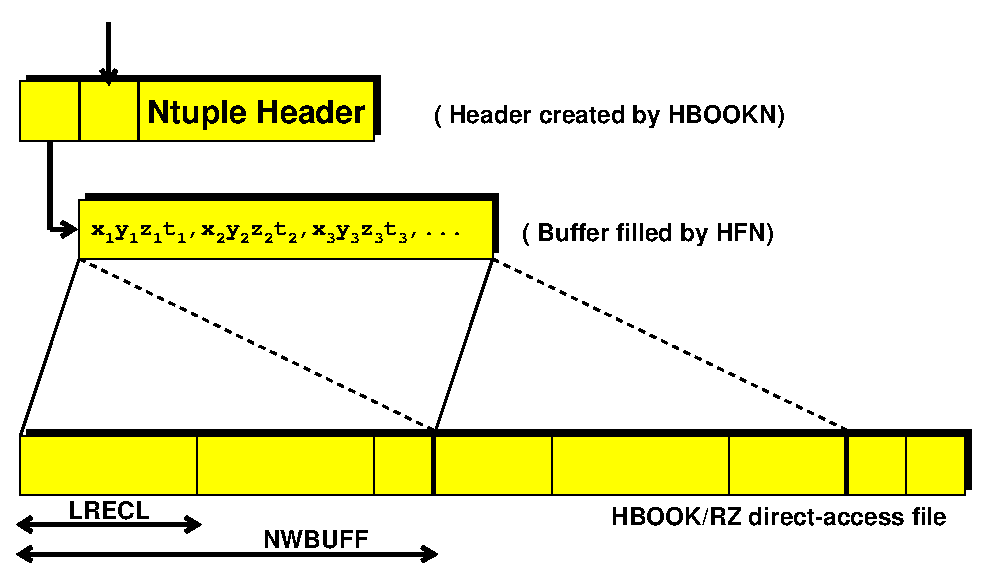
\epsfig{file=rwn.eps,width=.95\textwidth}}
\caption{Schematic structure of a RWN Ntuple}
\label{fig:rwn}
{\centering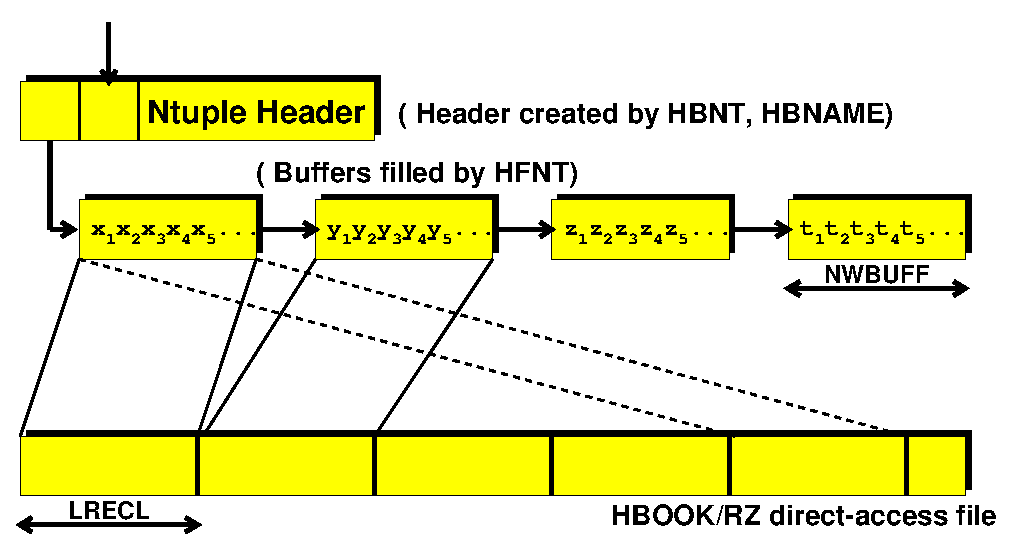
\epsfig{file=cwn.eps,width=.95\textwidth}}
\caption{Schematic structure of a CWN Ntuple}
\label{fig:cwn}
\newcommand{\III}{\(\sb{\mathtt{i}}\)}

\small

Figure~\ref{fig:cwn} shows the layout of a \CWN{} Ntuple.
The buffer size for each of the columns
\Lit{NWBUFF} was set equal to the record length \Rarg{LRECL}
(defined with routine \Rind{HROPEN}).
A \CWN{} requires a large value for the length of the common \Lit{/PAWC/},
\index{common {\tt/PAWC/}}\index{PAWC@{\tt/PAWC/} common}%
in any case larger than the number of columns
times the value \Lit{NWBUFF}, i.e. \Lit{NWPAWC>NWBUFF*NCOL}.
You can, however, expect important performance improvements by setting
the buffer size \Lit{NWBUFF} equal to a 
multiple of the record length \Rarg{LRECL} (via routine \Rind{HBSET}).

In both figures, \Lit{x\III}, \Lit{y\III}, \Lit{z\III}, 
\Lit{t\III}, etc. represent the columns of event \Lit{i}.

\end{figure}

\clearpage

\Filename{H2Row-Wise-Ntuples}
\section{Row-Wise-Ntuples (RWN)}
\label{sec:NtupleRWN}
\subsection{Booking a RWN}
\label{HNTUBOOK}
 
\Shubr{HBOOKN}{(ID,CHTITL,NVAR,CHRZPA,NWBUFF,CHTAGS)}
 
\Action Books a \RWN{} in memory or with
automatic overflow on an \Lit{RZ} file.
Only single precision floating point numbers (\Lit{REAL*4} on
32 bit machines) can be stored, no data compression is provided.

\begin{DLtt}{123456}
\item[{\rm\bf Input parameters:}]
\item[ID] Identifier of the Ntuple.
\item[CHTITL] Character
    variable containing the title associated with the Ntuple.
\item[NVAR] Number of variables per event (\Lit{NVAR\(\leq\)512})
\item[CHRZPA] Character variable containing the path
    name of a RZ file onto which the contents of the Ntuple
    can overflow.
    \begin{DLtt}{123456}
    \item[' '] {\bf Memory resident Ntuples:} \\
    \index{Ntuple!memory resident}%
        A bank of \Lit{NWBUFF} words is created.
        Further banks of the same size are added in a linear
        chain should additional space be required at filling time.
    \item['RZTOP'] {\bf Disk resident Ntuples:} (recommended) \\
    \index{Ntuple!disk resident}%
        A disk resident Ntuple is created if the \Lit{CHRZPA}
        argument specifies the top directory name of an existing RZ file
        that has already been opened with \Rind{HROPEN} or \Rind{HRFILE}.
        A bank of length \Lit{NWBUFF} is created, as in the case of 
        memory resident Ntuples. However, each time the bank becomes full
        it is automatically flushed to the RZ file, rather than
        creating additional banks in memory.
    \end{DLtt}
\item[NWBUFF]Number of words for the primary allocation for the Ntuple.
\item[CHTAGS] Character array of length \Lit{NVAR}, providing a short
    name (up to eight characters) tagging scheme for each variable.
\end{DLtt}
 
\begin{XMPt}{Example of the declaration of a memory resident RWN}
      CHARACTER*2 CHTAGS(5)
      DATA CHTAGS/'Px','Py','Pz','Q2','NU'/
 *
      CALL HBOOKN(10,'My first NTUPLE',5,' ',1000,CHTAGS)
\end{XMPt}
 
\subsection{Filling a RWN}
\label{HNTUFILL}

\Shubr{HFN}{(ID,X)}
 
\Action
Fills a \RWN{}.
 
\begin{DLtt}{123456}
\item[{\rm\bf Input parameters:}]
\item[ID] Identifier of the Ntuple.
\item[X] Array of dimension \Lit{NVAR} containing
the values for the current event.
\end{DLtt}
 
\subsection*{Memory resident Ntuples} 
\index{Ntuple!memory resident}

When a \RWN{} is booked, HBOOK reserves space in memory
in which to store the data, as specified by the \Rarg{NWBUFF}
argument of routine \Rind{HBOOKN}.
\index{memory}
As the \RWN{} is filled by a call to \Rind{HFN}, 
this space will be successively used until full. 
At that time, a new memory allocation will be made
and the process continues.

If this data is then written to disk, it appears as one
enormous logical record. 
In addition, it most cases the last block of data will 
not be completely filled thus wasting space.

If one tries to reprocess this \RWN{} at a later date,
e.g. with \PAW{}, there must be enough space in memory to
store the entire Ntuple. 
This often gives rise to problems
and so the following alternative method is recommended.

\subsection*{Circular buffer}
\index{circular buffer}

In an online environment you often want to have the last $N$ events
inside a buffer, so that the experiment can be monitored continuously.
To make it easier to handle this case, you can use routine \Rind{HFNOV},
which fills a circular buffer in memory with \RWN{} events, and when
the buffer is full, overwrites the oldest Ntuple.

\Shubr{HFNOV}{(ID,X)}
 
\Action
Fills a circular buffer with \RWN{}s.
 
\begin{DLtt}{123456}
\item[{\rm\bf Input parameters:}]
\item[ID] Identifier of the Ntuple.
\item[X] Array of dimension \Lit{NVAR} containing
the values for the current event.
\end{DLtt}

\subsection*{Disk resident Ntuples} 
\index{Ntuple!disk resident}

Prior to booking the \RWN{}, a new HBOOK RZ file is created
using \Rind{HROPEN}. 
The top directory name of this file is passed
to routine \Rind{HBOOKN} when the Ntuple is booked.

Filling proceeds as before but now, when the buffer in memory
is full, it is written to the HBOOK file and then reused
for the next elements of the Ntuple. 
This normally results in a more efficient 
utilisation of the memory,
both when the Ntuple is created and when it is reprocessed.

\begin{XMPt}{Recommended way of creating a RWN}
      PROGRAM TEST
      PARAMETER (NWPAWC = 15000)
      COMMON/PAWC/PAW(NWPAWC)
      CHARACTER*8 CHTAGS(5)
      DIMENSION EVENT(5)
      EQUIVALENCE (EVENT(1),X),(EVENT(2),Y),(EVENT(3),Z)
      EQUIVALENCE (EVENT(4),ENERGY),(EVENT(5),ELOSS)
      DATA CHTAGS/'X','Y','Z','Energy','Eloss'/
*
      CALL HLIMIT(NWPAWC)
      CALL HROPEN(1,'EXAMPLE','EXAMPLE.DAT','N',1024,ISTAT)
      IF(ISTAT.NE.0)GO TO 99
*
      CALL HBOOKN(10,'A Row-Wise-Ntuple',5,'//EXAMPLE',5000,CHTAGS)
      CALL HBOOK1(100,'Energy distribution',100,0.,100.,0.)
*
      DO 10 I=1,10000
         CALL RANNOR(X,Y)
         Z=SQRT(X*X+Y*Y)
         ENERGY=50. + 10.*X
         ELOSS=10.*ABS(Y)
         CALL HFN(10,EVENT)
         CALL HFILL(100,ENERGY,0.,1.)
 10   CONTINUE
*
      CALL HROUT(0,ICYCLE,' ')
      CALL HREND('EXAMPLE')
*
 99   CONTINUE
      END
\end{XMPt}

%\newpage%%%%%%%%%%%%%%%%%%%%%%%%%%%%%%%%%%%%%%%%%%%%%%%%%%%%%%%%%%

When the Ntuple is filled, routine \Rind{HFN} will
automatically write the buffer to the directory in the
RZ~file, which was specified in the call to \Rind{HBOOKN}
(the top directory \Lit{//EXAMPLE} in the example above).
If the current directory (CD)\index{current directory}\index{directory!current}
is different, \Rind{HFN} will save and
later automatically restore the CD.

The Ntuple created by the program shown above can be processed
by \PAW{} as follows.

\begin{XMPt}{Reading an RWN in a PAW session}
            PAW > Histo/file  1  example.dat
            PAW > Histo/plot 100
            PAW > Ntuple/plot 10.energy
            PAW > Ntuple/plot 10.eloss  energy<50
            PAW > Ntuple/plot 10.eloss%energy  x<2.and.sqrt(z)>1
\end{XMPt}

By default \Rind{HROPEN} creates a file that can be extended up to
32000 blocks, i.e. 128 Mbytes for a record length \Lit{LREC}
of 1024 words.
If one wishes to create very large Ntuples, one should
make two changes to the above procedure.

\begin{UL}
\item A large value should be used for the record length of the file,
      e.g. 8192 words (the maximum on most machines).
      {\bf N.B. the maximum record length on VMS systems is 8191 words.
      If RELATIVE access mode is used, the maximum is then 4095 words.}
      This remark does not apply to a \CWN, as described later.
\item Option \Lit{Q} on \Rind{HROPEN} should be used to override the default
      number of records allowed. 
\end{UL}

This can be achieved as by changing the previous call to \Rind{HROPEN}
as follows:

\begin{XMPt}{Writing very large Ntuple files}
              COMMON/QUEST/IQUEST(100)
              CALL HLIMIT(150000)
*
*     Create HBOOK file with the maximum record length (32756 bytes)
*     and maximum number of records (65000)
*
              IQUEST(10) = 65000
              CALL HROPEN(1,'EXAMPLE','EXAMPLE.DAT','NQ',8192,ISTAT)
              IF(ISTAT.NE.0)GO TO 99
\end{XMPt}
\index{IQUEST@{\tt IQUEST} communication vector}

\newpage%%%%%%%%%%%%%%%%%%%%%%%%%%%%%%%%%%%%%%%%%%%%%%%%%%%%%%%%%%

\Filename{H2More-general-Ntuples}
\section{More general Ntuples: Column-Wise-Ntuples (CWN)}
\label{sec:NtupleCWN}

A \CWN{} supports the storage of the following data types: floating
point numbers (\Lit{REAL*4} and \Lit{REAL*8}), integers, bit patterns
(unsigned integers), booleans and character strings.

\subsection*{Data Compression}

Floating point numbers, integers and bit patterns can be packed by
specifying a range of values or by explicitly specifying the number
of bits that should be used to store the data. Booleans are always
stored using one bit. Unused trailing array elements will not be
stored when an array depends on an index variable. In that case only
as many array elements will be stored as specified by the index
variable.

For example, the array definition \Lit{NHITS(NTRACK)} 
defines \Lit{NHITS} to depend on the index variable \Lit{NTRACK}. 
When \Lit{NTRACK} is 16, the elements \Lit{NHITS(1..16)} are stored, 
when \Lit{NTRACK} is 3, only elements \Lit{NHITS(1..3)} are stored, etc.

\subsection*{Storage Model}

Column wise storage allows direct access to any column in the Ntuple. 
Histogramming one column from a 300 column \CWN{} requires reading 
only 1/300 of the total data set. 
However, this storage scheme requires one memory buffer per column 
as opposed to only one buffer in total for an \RWN.
By default the buffer length is 1024 words, 
in which case a 100 column Ntuple requires 409600 bytes of buffer space. 
In general, performance increases with buffer size.
Therefore, one should tune the buffer size (using routine \Rind{HBSET}) 
as a function of the number of columns and the amount of available memory.
Highest efficiency is obtained when setting the buffer size equal to the
record length of the RZ HBOOK file (as specified in the call to
\Rind{HROPEN}). 
A further advantage of column wise storage is that a \CWN{}
can easily be extended with one or more new columns.

Columns are logically grouped into blocks (physically, however, all
columns are independent). 
Blocks allow users to extend a \CWN{} with private columns or to 
group relevant columns together.
New blocks can even be defined after a \CWN{} has been filled. 
The newly created blocks can be filled using routine \Rind{HFNTB}.
For example, a given experiment might define a number of standard
Ntuples. These would be booked in a section of the code that
would not normally be touched by an individual physicist. However,
with a \CWN{} a user may easily add one or more blocks of information
as required for their particular analysis.

Note that arrays are treated as a single column. 
This means that a \CWN{} will behave like a \RWN{},
with the addition of data typing and compression,
if only one array of \Lit{NVAR} elements is declared.
This is not recommended as one thereby loses
the direct column access capabilities of a \CWN{}.

\subsection*{Performance}

Accessing a relatively small number of the total number of
defined columns results in a huge increase in performance compared to
a \RWN{}.
However, reading a complete \CWN{} will take
slightly longer than reading a \RWN{} due to the overhead
introduced by the type checking and compression mechanisms and
because the data is not stored sequentially on disk.  
The performance increase with a \CWN{} will most clearly show up when 
using \PAW{}, where one typically histograms one
column with cuts on a few other columns.  
The advantages of having different data types and data compression generally
outweighs the performance penalty incurred when reading a complete \CWN{}.

\newpage%%%%%%%%%%%%%%%%%%%%%%%%%%%%%%%%%%%%%%%%%%%%%%%%%%%%%%%%%%

\subsection{Booking a CWN}
\label{HNTUBOOKT}

The booking is performed in two stages. 
Firstly, a call to \Rind{HBNT}
is made to declare the Ntuple identifier and title. 
Secondly, one or more
calls are made to \Rind{HBNAME} or \Rind{HBNAMC} to describe 
the variables that are to be stored in the Ntuple. 
Routine \Rind{HBNAMC} is used to define \Lit{CHARACTER} variables,
while all other variable types are defined with routine \Rind{HBNAME}.

\Shubr{HBNT}{(ID,CHTITL,CHOPT)}

\Action
Books a \CWN.
 
\begin{DLtt}{12345678}
\item[{\rm\bf Input parameters:}]
\item[ID]     Identifier of the Ntuple.
\item[CHTITL] Character variable specifying the title associated to the Ntuple.
\item[CHOPT]  Character variable specifying the desired options.
   \begin{DLtt}{123}
     \item[' '] for disk resident Ntuples (default).
     \item['D'] idem as \Lit{' '}.
     \item['M'] for memory resident Ntuples.
   \end{DLtt}
\end{DLtt}

The CWN{} will be stored in the current HBOOK directory.
The variables to be stored in the Ntuple will be specified
with routine \Rind{HBNAME} or \Rind{HBNAMC} described below.

When the \CWN{} will be filled with \Rind{HFNT}, the memory buffers associated 
with each column will be written to the file and directory corresponding 
to the current working directory when \Rind{HBNT} was called.
Remember that when routine \Rind{HROPEN} is called, the current
working directory is automatically set to the
top directory of that file.
It is therefore convenient to call \Rind{HBNT} immediately after \Rind{HROPEN}.
If this was not the case, routine \Rind{HCDIR} must be called prior to
\Rind{HBNT} to set the current working directory.
When the Ntuple has been filled (via calls to \Rind{HFNT})
the resident buffers in memory as well as the Ntuple header 
must be written to the file with a call to \Rind{HROUT}.
Before calling \Rind{HROUT}, the current working directory 
must be set to the current directory when \Rind{HBNT} was called.

\Shubr{HBSET}{(CHOPT,IVAL,IERR*)}

\Action
Set global Ntuple options.

\begin{DLtt}{123456}
\item[{\rm\bf Input parameters:}]
\item[CHOPT] Character variable specifying the parameter to set.
   \begin{DLtt}{1234567}
     \item['BSIZE'] Set the buffer size. For each variable (i.e.\ column)
                    a buffer of \Lit{BSIZE} words is created in memory.
                    The default for \Lit{BSIZE} is 1024.
   \end{DLtt}
\item[IVAL]   Value for the parameter specified with \Rarg{CHOPT}.
\item[{\rm\bf Output parameters:}]
\item[IERR]   Error return code (\Lit{=0} means no errors).
\end{DLtt}

If the total memory in \Lit{/PAWC/},
\index{common {\tt/PAWC/}}\index{PAWC@{\tt/PAWC/} common}%
allocated via \Rind{HLIMIT}
is not sufficient to accomodate all the column buffers of \Rarg{BSIZE} words,
then \Rind{HBNT} will automatically reduce the buffer size in such a way that all buffers can fit into
memory.
It is strongly recommended to allocate enough memory to \Lit{/PAWC/}
in such a way that each column buffer is at least equal to the block size of
the file.
A simple rule of thumb in the case of no data compression is to have 
\mbox{\Lit{NWPAWC>NCOL*LREC}}, where \Lit{NWPAWC}
is the total number of words allocated
by \Rind{HLIMIT}, \Lit{LREC} is the block size of the file in machine words
as given in the call to \Rind{HROPEN}  and \Lit{NCOL} is the number of columns.

\newpage%%%%%%%%%%%%%%%%%%%%%%%%%%%%%%%%%%%%%%%%%%%%%%%%%%%%%%%%%%

\subsection{Describing the columns of a CWN}
\label{HNTUDESC}

\Shubr{HBNAME}{(ID, CHBLOK, VARIABLE, CHFORM)}

\Shubr{HBNAMC}{(ID, CHBLOK, VARIABLE, CHFORM)}
\Action
Describe the variables to be stored in a \CWN{}
(non-character and character variables, respectively).
 
\begin{DLtt}{12345678}
\item[{\rm\bf Input parameters:}]
\item[ID]     Identifier of the Ntuple as in the call to \Rind{HBNT}.
\item[CHBLOK] Character variable of maximum length 8 characters 
              specifying the name by which the block
              of variables described by \Lit{CHFORM} is identified.
\item[VARIABLE] 
              The first variable that is described in \Lit{CHFORM}.
              Variables must be in common blocks but may not be
              in a ZEBRA bank.
              For example, given the common block \Lit{CEXAM} described
              below, one would call \Lit{HBNAME} with the argument \Lit{IEVENT}.
              In the case of character variables, the routine
              \Lit{HBNAMC} must be used. In all other cases one 
              should use \Lit{HBNAME}. 
\item[CHFORM] Can be either a character string describing the variables
              to be stored in block \Lit{CHBLOK} or:
   \begin{DLtt}{1234567}
     \item['\$CLEAR'] To clear the addresses of all variables in the Ntuple.
     \item['\$SET'] To set the addresses in which to write the values of
                    all variables in block \Lit{CHBLOK}.
   \end{DLtt}
             The last two forms are used before reading back the Ntuple data
             using \Rind{HGNT}, \Rind{HGNTB}, \Rind{HGNTV} or \Rind{HGNTF}.
             See also \Rind{HUWFUN}.
\end{DLtt}

With \Lit{CHFORM} the variables, their type, size and, possibly, range
(or packing bits) can all be specified at the same time. 
{\bf Note however that variable names should be unique, even when
they are in different blocks.}.
In the simplest
case \Lit{CHFORM} corresponds to the COMMON declaration. For example:
\begin{XMP}
       COMMON /CEXAM/ IEVENT, ISWIT(10), IFINIT(20), NEVENT, NRNDM(2)
\end{XMP}
can be described by the following \Lit{CHFORM}:
\begin{XMP}
       CHFORM = 'IEVENT, ISWIT(10), IFINIT(20), NEVENT, NRNDM(2)'
\end{XMP}
in this case the Fortran type conventions are followed and the default
sizes are taken, no packing is done. Note that to get a nice one-to-one
correspondance between the COMMON and the \Lit{CHFORM} statements
the dimension of the variables are specified in the COMMON and not
in a DIMENSION statement.

The default type and size of a variable can be overridden by
extending the variable name with \Lit{:<t>*<s>}:

\begin{tabular}{@{}>{\tt}cllcl}
\Lit{<t>} & type of variable & \Lit{<s>} values & default & routine      \\[1mm]
 R        & floating-point   & 4, 8             & 4       & \Rind{HBNAME}\\
 I        & integer          & 4, 8             & 4       & \Rind{HBNAME}\\
 U        & unsigned integer & 4, 8             & 4       & \Rind{HBNAME}\\
 L        & logical          & 4                & 4       & \Rind{HBNAME}\\
 C        & character        & \tt[4$\le$s$\le$32] (multiple of 4)
                                                & 4       & \Rind{HBNAMC}\\
\end{tabular}

\newpage%%%%%%%%%%%%%%%%%%%%%%%%%%%%%%%%%%%%%%%%%%%%%%%%%%%%%%%%%%

When the range of a type \Lit{U}, \Lit{I} or \Lit{R} variable is known, its
storage size (number of packing bits) may be added behind
the \Lit{:<t>*<s>} specification using \Lit{:<b>} for types \Lit{U}
and \Lit{I} and \Lit{:<b>:[<min>,<max>]} for type \Lit{R}. 
Floating-points are packed into an integer using:
\begin{XMP}
IPACK = ((R - <min>)/(<max> - <min>)*(2**<b> - 1) + 0.5
\end{XMP}

When \Lit{:<b>...} is not specified a variable is stored using the
number of bytes given by \Lit{<s>} or the default. 
In case the default type and size of a variable should be used, the
packing bits can be specified as \Lit{::<b>...}. 
\Lit{<b>} must be in the range \Lit{1}\(\le\)\Lit{b}\(\le\)\Lit{8*<s>}.
Automatic bit packing will happen, for type \Lit{U} and \Lit{I}, when a range
is specified like: \Lit{ICNT[-100,100]}. In this case \Lit{ICNT} will
be packed in 8 bits (7 bits for the integer part and 1 bit for the sign).
In case \Lit{CNT} is an integer ranging from -100 to 100 it could be
specified either like \Lit{CNT[-100,100]:I} or like \Lit{CNT:I::[-100,100]}.
Logical variables will always be stored in 1 bit.
All variables must be aligned on a word boundary and character variables
must have a length modulo 4. The maximum length of the variable name
is 32 characters.

Variable-length Ntuple rows and looping over array components
are also supported to optimize Ntuple storage and Ntuple plotting.
Variable row length can occur when arrays in the Ntuple
depend on an index variable.

\begin{XMPt}{Example of a variable row length CWN definition}
      PARAMETER (MAXTRK = 100, MAXHIT = 300)
      COMMON /CMTRK/ NTRACK, NHITS(MAXTRK), PX(MAXTRK), PY(MAXTRK),
     +               PZ(MAXTRK), XHITS(MAXHIT,MAXTRK), YHITS(MAXHIT,MAXTRK),
     +               ZHITS(MAXHIT,MAXTRK)
      CALL HBNAME(ID,'VARBLOK2',NTRACK, 
     +            'NTRACK[0,100], NHITS(NTRACK)[0,300],'//
     +            'PX(NTRACK), PY(NTRACK), PZ(NTRACK), XHITS(300,NTRACK),'//
     +            'YHITS(300,NTRACK), ZHITS(300,NTRACK)')
\end{XMPt}

In this example the number of elements to store in one Ntuple row
depends on the number of tracks, \Lit{NTRACK}.
The call to \Rind{HBNAME} declares \Lit{NTRACK} to be an
index variable and that the size of the Ntuple row depends on the value of 
this index variable.
The range of an index variable is specified using \Lit{[<l>,<u>]},
where \Lit{<l>} is the lower and \Lit{<u>} the upper limit of the arrays
using this index variable. In the above example the 
lower limit of \Lit{NTRACK} is 0 and the upper limit is 100 (\Lit{= MAXTRK}).
While filling a \CWN{} HBOOK can also easily test for
array out-of-bound errors since it knows the range of \Lit{NTRACK}.
Only the last dimension of a multi-dimensional array may be variable
and the index variable must be specified in the block where it is used.
Array lower bounds must, just like the lower range of the index variable,
be 0.

\Rind{HBNAME} may be called more than once per block as long as no data
has been stored in the block. 
New blocks can be added to an Ntuple at any time, even after filling has started,
whereas existing blocks may only be extended before filling has started.
\index{block}


\subsection*{Alternative way of booking a CWN}

\Shubr{HBOOKNC}{(ID,CHTITL,NVAR,BLOCK,TUPLE,CHTAGS)}

\Action Provides a way to define a \CWN{} similar to 
\Rind{HBOOKN} for a \RWN{}.

\begin{DLtt}{123456}
\item[{\rm\bf Input parameters:}]
\item[ID] Identifier of the CWN{}.
          If it does not already exist, it is created.
\item[CHTITL] Character variable specifying the name of the Ntuple
          (not used if it already exists).
\item[NVAR]  Number of variables per event (maximum 200).
\item[BLOCK] Name of the block inside the \CWN (default is \Lit{'Block1'}.
\item[TUPLE] Array of dimension \Lit{NVAR} that will contain values at filling
                 time.
\item[CHTAGS] Character array of length \Lit{NVAR}, providing a short
    name (up to eight characters) tagging scheme for each variable.
\end{DLtt}

\subsection{Filling a CWN}
\label{HNTUFILLT} 

\Shubr{HFNT}{(ID)}
 
\Action Fill a \CWN{}.
 
\begin{DLtt}{123456}
\item[{\rm\bf Input parameter:}]
\item[ID] Identifier of the CWN{}.
\end{DLtt}
\Rind[HROPEN]{}
\Rind[HBNT]{}
\Rind[HBNAME]{}
\Rind[HBNAMC]{}
\Rind[HFNT]{}
\Rind[HROUT]{}
\Rind[HREND]{}
\index{PAW}


\Shubr{HFNTB}{(ID,CHBLOK)}
 
\Action Fill the named block \Lit{CHBLOK} in a \CWN{}.
 
\begin{DLtt}{123456}
\item[{\rm\bf Input parameters:}]
\item[ID] Identifier of the Ntuple.
\item[CHBLOK]Character variable specifying the block that is to be filled.
\end{DLtt}

\Shubr{HPRNT}{(ID)}
 
\Action Print the  definition of the CWN{} \Lit{ID} as 
defined by the calls to \Rind{HBNAME} and/or \Rind{HBNAMC}.
 
\begin{DLtt}{123456}
\item[{\rm\bf Input parameter:}]
\item[ID] Identifier of the CWN{}.
\end{DLtt}

\subsection*{Recovery procedure}
\label{sec:Ntuple-recovery}

The Ntuple header, containing the essential
definitions associated with an Ntuple,
are now written to the output file when the first
buffer is written. 
If the job producing the Ntuple does not terminate in a clean way 
(i.e. the job crashs or you forgot to call \Rind{HROUT}), 
it is now possible to rebuild the Ntuple header from the 
information available in the file.
Note, however, that the events corresponding to the last 
Ntuple buffer in memory are lost.

\Shubr{HRECOV}{(ID,CHOPT)}

\Action Recover the information associated with a \CWN{}.
 
\begin{DLtt}{123456}
\item[{\rm\bf Input parameters:}]
\item[ID]    Identifier of the CWN{}.
\item[CHOPT] Character variable specifying the option desired.
             At present Not used at present; \Lit{' '}
             should be specified
\end{DLtt}

\newpage%%%%%%%%%%%%%%%%%%%%%%%%%%%%%%%%%%%%%%%%%%%%%%%%%%%%%more com

\begin{XMPt}{Example of saving contents of common variables in an Ntuple}
        COMMON/GCFLAG/IDEBUG,IDEMIN,IDEMAX,ITEST,IDRUN,IDEVT,IEORUN
       +        ,IEOTRI,IEVENT,ISWIT(10),IFINIT(20),NEVENT,NRNDM(2)

        COMMON/GCTRAK/VECT(7),GETOT,GEKIN,VOUT(7),NMEC,LMEC(MAXMEC)
       + ,NAMEC(MAXMEC),NSTEP ,MAXNST,DESTEP,DESTEL,SAFETY,SLENG
       + ,STEP  ,SNEXT ,SFIELD,TOFG  ,GEKRAT,UPWGHT,IGNEXT,INWVOL
       + ,ISTOP ,IGAUTO,IEKBIN, ILOSL, IMULL,INGOTO,NLDOWN,NLEVIN
       + ,NLVSAV,ISTORY

        COMMON/GCTMED/NUMED,NATMED(5),ISVOL,IFIELD,FIELDM,TMAXFD,DMAXMS
       +      ,DEEMAX,EPSIL,STMIN,CFIELD,PREC,IUPD,ISTPAR,NUMOLD

        CHARACTER*4 TYPE
        COMMON/CMCC/TYPE

*     The code to book and fill the Ntuple would look like this:
*
*   Initialisation phase.
*   The calls to HROPEN, HBNT and HBNAME may be placed in different 
*   initialisation routines. 
*   In this example example the Ntuple will be stored in directory //MYFILE.
*
        CALL HROPEN(1,'MYFILE','geant.ntup','N',1024,ISTAT)
        CALL HBNT(10,'Geant Ntuple',' ')
*
        CALL HBNAME(10, 'RUN',    IDRUN,  'IDRUN::16,IDEVT::16')
        CALL HBNAME(10, 'RUN',    IEORUN, 'IEORUN::16')
        CALL HBNAME(10, 'VECT',   VECT,   'VECT(6)')
        CALL HBNAME(10, 'GEKIN',  GEKIN,  'GEKIN')
        CALL HBNAME(10, 'INWVOL', INWVOL, 'INWVOL[1,7],ISTOP[1,7]')
        CALL HBNAME(10, 'NUMED',  NUMED,  'NUMED::10')
        CALL HBNAME(10, 'NSTEP',  NSTEP,  'NSTEP::16')
        CALL HBNAMC(10, 'TYPE',   TYPE,   'TYPE:C')
*
*    To fill the Ntuple, when the common blocks are filled just invoke
*    routine HFNT which knows the addresses and the number of variables.
*
        DO 10 I = 1, 1000000
           ...
           CALL HFNT(10)
10      CONTINUE
*
*                      At the end of the job, proceed as usual
*
        CALL HROUT(10, ICYCLE, ' ')
        CALL HREND('MYFILE')

\end{XMPt}

\newpage%%%%%%%%%%%%%%%%%%%%%%%%%%%%%%%%%%%%%%%%%%%%%%

\begin{changebar}
\subsection*{Disk resident Ntuples}

Histograms are never created directly on a disk file. 
They are always created in the current directory in memory 
(\Lit{//PAWC} or \Lit{//PAWC/subdir}).
Histograms are saved on the disk file with a call of type 
\Lit{CALL \Rind{HROUT}}
In case of disk-resident Ntuples, it is the same thing. 
The Ntuple header 
(data structure containing the column names) is always created
in the current directory in memory 
(\Lit{//PAWC} or \Lit{//PAWC/subdir}).
However, the call to \Rind{HBNT} remembers the current 
directory on disk (in the case below
the \Lit{CD} on disk is \Lit{//K0}). 
When you fill the Ntuple, \Rind{HFNT} fills a buffer in memory. 
When this buffer is full, \Rind{HFNT} knows what is the \Lit{CD} on disk.
The buffer is written into that directory. 
Note that your current directory on disk may be somewhere else. 
\Rind{HFNT} will temporarely change the \Lit{CD} to \Lit{//K0} 
and will reset the \Lit{CD} to what it was before calling \Rind{HFNT}.
At the end of your job, you have to save the header and the current buffer
in memory on the disk file. 
For that you have to:

\begin{UL}
\item[--] Change the directory in memory where you book the ntuple. 
          If you do not have subdirectories, 
          this operation is not necessary.
\item[--] Change the directory on disk where you specified it in 
          \Rind{HBNT}. 
          In the case below \Lit{//KO}.
\item[--] Issue a call to \Rind{HROUT} or \Rind{HREND}.
\end{UL}

\begin{XMPt}{Creating a disk resident Ntuple}
      call HCDIR('//PAWC',' ')
*--     HROPEN sets the directory to //K0, so no call to HCDIR is needed
      call HROPEN(50,'K0','~/mydir/K0.rz','N',1024,ISTAT)
      if (ISTAT.ne.0) write(6,*) 'Error in HROPEN'
      call HBNT(1000,'NTuple','D')
      call HLDIR('//PAWC','T') ! Now you can see the header in //PAWC
      call HLDIR('//K0','T')   ! OK, nothing yet on //K0
*--     HBNAME describes the Ntuple
      call HBNAME(1000,'Event',EvtNo,
     +            'RunNo:I,Evtno:I,NPos:I,NNeg:I,'//
     +            ....
....
        call HLDIR('//K0','T') ! Nothing yet on //K0
        call HCDIR('//K0',' ') ! Useless, HFNT remembers that buffers are written to //KO
        call HFNT(1000)
        call HLDIR(' ','T')    ! This will not show anything on //K0.
                               ! However if you call HLDIR(' ','TA') you will see all Ntuple 
                               ! extensions in the case you have many calls to HFNT. 
                               ! In this particular example everything is still in memory.
....
      call HCDIR('//K0',' ')   ! Useless, you are already here
      call HLDIR('//K0',' ')   ! same as call hldir(' ','T')
      call RZLDIR(' ',' ')
      call HROUT(0,icycle,' ')
*-*      If you call HLDIR(' ',' ') here you will see the header
*-*      If you call HLDIR(' ','A') here you will see the header and your Ntuple extensions
      call HREND('K0')
\end{XMPt}
\end{changebar}

\newpage%%%%%%%%%%%%%%%%%%%%%%%%%%%%%%%%%%%%%%%%%%%%%%

\Filename{H2Making-projection-of-a-RWN}
\section{Making projections of a RWN}
\label{HNTUPROJ} 

\Shubr{HPROJ1}{(ID,IDN,ISEL,FUN,IFROM,ITO,IVARX)}
 
\Action
Fill an existing one-dimensional histogram with data from a RWN.
 
\begin{DLtt}{123456}
\item[{\rm\bf Input parameters:}]
\item[ID]    Identifier of a 1-dimensional histogram, which
             must have been previously booked with \Rind{HBOOK1}.
\item[IDN]   Identifier of the RWN Ntuple.
\item[ISEL]  Selection flag
             \begin{DLtt}{1234}
                \item[0]   No selection criterion. All events between \Lit{IFROM} and
                           \Lit{ITO} are histogrammed with a weight of one.
                \item[<>0] The function \Lit{FUN} is called for each event
                           between \Lit{IFROM} and \Lit{ITP}, which are histogrammed
                           with as weight the value of \Lit{FUN}. of one.
             \end{DLtt}
\item[FUN]   User function, to be declared \Lit{EXTERNAL} in the calling
             routine. It has as parameters the array of variables \Lit{X} and the
             selection flag \Lit{ISEL}. If \Lit{FUN=0.},
             no filling takes place for that event.
\item[IFROM] Event number where the histogramming has to start.
\item[ITO]   Event number where the histogramming has to end.
\item[IVARX] Sequence number in the Ntuple of the variable to be
             histogrammed
\end{DLtt}

\begin{XMPt}{Example of the use of a one-dimensional Ntuple projection}
     PROGRAM MAIN
     EXTERNAL WFUNC
     CALL HPROJ1(10,20,1,WFUNC,0,0,4)
     .....

     FUNCTION WFUNC(X,ISEL)
     DIMENSION X(*)
     WFUNC=0.
     IF(ISEL.EQ.1)THEN
         IF(X(2)**2 +X(3)**2.LT.0.)WFUNC=1.
     ELSEIF(ISEL.EQ.2)THEN
         IF(X(2)**2 +X(3)**2.GT.5.)WFUNC=1.
     ELSE
         WFUNC=X(5)
     ENDIF
     END
\end{XMPt}

Note that in an interactive session with \PAW{},
the user function \Lit{FUN} can be defined
interactively using a Fortran-like syntax without recompilation
and relinking.
 
\Shubr{HPROJ2}{(ID,IDN,ISEL,FUN,IFROM,ITO,IVARX,IVARY)}
 
\Action
Same action as \Rind{HPROJ1}, but filling a previously
booked 2-dimensional histogram or a profile histogram.
Variable \Lit{X(IVARX)} will be projected onto the \Lit{X} axis and
\Lit{X(IVARY)} onto the \Lit{Y} axis for all entries in the Ntuple
between \Lit{IFROM} and \Lit{ITO} inclusive.
 
The number of entries in an Ntuple can be obtained by \Rind{HNOENT}.
 
\newpage%%%%%%%%%%%%%%%%%%%%%%%%%%%%%%%%%%%%%%%%%%%%%%%%%%%%%%%%%%%%%%%

\Filename{H2Get-information-about-an-Ntuple}
\section{Get information about an Ntuple}
 
\Shubr{HGIVEN}{(ID,CHTITL*,*NVAR*,CHTAG*,RLOW*,RHIGH*)}
 
\Action
Routine to provide information about an Ntuple.
 
\begin{DLtt}{123456}
\item[{\rm\bf Input parameters:}]
\item[ID] Identifier of the Ntuple.
\item[NVAR] Dimension of arrays \Lit{TAGS}, \Lit{RLOW}
and \Lit{RHIGH}.
\item[{\rm\bf Output parameters:}]
\item[CHTITL] Character
variable containing the title associated with the Ntuple.
\item[NVAR] The original contents is overwritten by the actual dimension of the Ntuple.
If \Lit{ID1} does not exist or is not an Ntuple \Lit{NVAR=0} is returned.
\item[CHTAG] Character array of dimension \Lit{NVAR}, which
contains the tag names of the Ntuple elements.
\item[RLOW] Array of dimension \Lit{NVAR}, which
contains the lowest value for each Ntuple element.
\item[RHIGH] Array of dimension \Lit{NVAR}, which
contains the highest value for each Ntuple element.
\end{DLtt}
 
\subsection{Retrieve the contents of a RWN into an array}
 
\Shubr{HGN}{(ID,*IDN*,IDNEVT,X*,IERROR*)}
 
\Action
Copy the contents of a \RWN{} event into an array.
 
\begin{DLtt}{123456}
\item[{\rm\bf Input parameters:}]
\item[ID]     Identifier of the Ntuple.
\item[IDN]    Must be initialized to zero before the first call to \Rind{HGN}.
\item[IDNEVT] Event number
\item[{\rm\bf Output parameters:}]
\item[IDN]    Internal HBOOK pointer
\item[X]      Array to contain variables for the event chosen.
\item[IERROR] Error return code.
\end{DLtt}

This routine returns in the vector \Lit{X} the contents of the 
row \Lit{IDNEVT} or Ntuple \Lit{ID}. 
The vector \Lit{X} must be of size \Lit{NVAR},
as specified in the call to \Rind{HBOOKN}.
If more than one row of the Ntuple is to be processed, it is more
efficient to call first \Rind{HGNPAR} and then \Rind{HGNF}.

\Shubr{HGNPAR}{(ID,CHROUT)}

\Action
Obtains the address and parameters of Ntuple ID.
\begin{DLtt}{123456}
\item[{\rm\bf Input parameters:}]
\item[ID]Identifier of the Ntuple.
\item[CHROUT]Character variable containing the name of the calling
subroutine (printed in case of errors).
\end{DLtt}

This routine sets some internal pointers and must be called before
the first call to \Rind{HGNF} for a given \RWN{}. When accessing
more than one row of an Ntuple it is more efficient to call
\Rind{HGNPAR} and then \Rind{HGNF} for each row that is required
than to call \Rind{HGN}.

\Shubr{HGNF}{(ID,IDNEVT,X*,IERROR*)}
 
\Action
Copy the contents of an Ntuple event into an array.
The routine \Rind{HGNPAR} must have been called
prior to the first call to \Rind{HGNF} for a given
Ntuple.
 
\begin{DLtt}{123456}
\item[{\rm\bf Input parameters:}]
\item[ID]Identifier of the Ntuple.
\item[IDNEVT]Event number
\item[{\rm\bf Output parameters:}]
\item[X] Array to contain variables for the event chosen.
\item[IERROR] Error return code.
\end{DLtt}

This routine returns in the vector \Lit{X} the contents of the 
row \Lit{IDNEVT} or Ntuple \Lit{ID}. 
The vector \Lit{X} must have be of size \Lit{NVAR},
as specified in the call to \Rind{HBOOKN}.

\begin{XMPt}{Example of access to RWN information}
\NODOC{\baselineskip=.95\baselineskip\relax}      PROGRAM TEST
      INTEGER    NWPAWC
      PARAMETER (NWPAWC=15000, MTUPLE=5)
      COMMON/PAWC/PAW(NWPAWC)
      CHARACTER*80 CHTITL
      CHARACTER*8 CHTAGS(MTUPLE),CHTAGZ(MTUPLE)
      DIMENSION EVENT(MTUPLE),RLOW(MTUPLE),RHIGH(MTUPLE)
      EQUIVALENCE (EVENT(1),X),(EVENT(2),Y),(EVENT(3),Z)
      EQUIVALENCE (EVENT(4),ENERGY),(EVENT(5),ELOSS)
      DATA CHTAGS/'X','Y','Z','Energy','Eloss'/
*-- Tell HBOOK how many words are in PAWC.
      CALL HLIMIT(NWPAWC)
*-- Book Ntuple 
      CALL HBOOKN(10,'A Row-Wise-Ntuple',5,' ',5000,CHTAGS)
*-- Fill the Ntuple 
      DO 10 I=1,1000
         CALL RANNOR(X,Y)
         Z=SQRT(X*X+Y*Y)
         ENERGY=50. + 10.*X
         ELOSS=10.*ABS(Y)
         CALL HFN(10,EVENT)
 10   CONTINUE
*--   Obtain the definitions of the Ntuple
      NVAR = MTUPLE
      CALL HGIVEN(10,CHTITL,NVAR,CHTAGZ,RLOW,RHIGH)
      PRINT *,'Definitions of Ntuple # ',10
      PRINT *,'   Title: ',CHTITL(1:LENOCC(CHTITL))
      PRINT *,'   Number of variables: ',NVAR
      DO 20 I=1,NVAR
         PRINT 9001,I,RLOW(I),RHIGH(I)
9001  FORMAT(' Min/Max values for column # ',I3,1X,F10.5,
     +       1X,F10.5)
 20   CONTINUE
*--   Get the contents of 'event' # 333
      CALL HGNPAR(10,'TEST')
      CALL HGNF(10,333,EVENT,IERR)
      PRINT *,IERR,EVENT
*--   Get the number of events in this Ntuple
      CALL HNOENT(10,NEVENT)
      PRINT *,NEVENT
 99   CONTINUE
      END
\end{XMPt}

\newpage%%%%%%%%%%%%%%%%%%%%%%%%%%%%%%%%%%%%%%%%%%%%%%%%%%%%%%%%%%

\subsection{Retrieve the contents of a CWN into a common block}
 
\Shubr{HGNT}{(ID,IDNEVT,IERR*)}
 
\Action

Retrieve information about a \CWN{} row.
 
\begin{DLtt}{123456}
\item[{\rm\bf Input parameters:}]
\item[ID] Identifier of the Ntuple.
\item[IDNEVT] Number of the event about which information is required.
\item[{\rm\bf Output parameter:}]
\item[IERR] Error return code (\Lit{=0} if event was found)
\end{DLtt}

The information is restored at the addresses specified by \Rind{HBNAME}
or \Rind{HBNAMC} (for \Lit{CHARACTER} data).
If the information is being retrieved by a program other than the
one that wrote the Ntuple then \Rind{HBNAME}
or \Rind{HBNAMC} must be called as appropriate (see below).
\begin{XMP}
      CALL HBNAME(ID,' ',0,'$CLEAR')
      CALL HBNAME(ID,CHBLOK,VARIABLE,'$SET')
\end{XMP}
\Rind[HBNAME]{}
\Rind[HBNAMC]{}
These calls are required as \Lit{HBOOK} must obtain the location
at which the requested information is to be returned which is
obviously not valid between programs.
The first call clears all the addresses stored by \Lit{HBOOK}
for the specified Ntuple and the second one sets the
addresses for the variables in block \Lit{CHBLOK} starting at variable
\Lit{VARIABLE}. The second call should be repeated for every block of
which data has to be retrieved. The routine \Rind{HUWFUN} will generate
these calls automatically in the skeleton user function.

\Shubr{HGNTB}{(ID,CHBLOK,IROW,IERR*)}
 
\Action

Retrieve information about a named block in an Ntuple row.
 
\begin{DLtt}{123456}
\item[{\rm\bf Input parameters:}]
\item[ID] Identifier of the Ntuple.
\item[CHBLOK]Character variable specifying the block that is to be
retrieved.
\item[IROW] Number of the row about which information is required.
\item[{\rm\bf Output parameter:}]
\item[IERR] Error return code (\Lit{=0} if row was found)
\end{DLtt}

The information is restored at the addresses specified by \Rind{HBNAME}
or \Rind{HBNAMC} (for \Lit{CHARACTER} data).

\Shubr{HGNTV}{(ID,CHVAR,NVAR,IROW,IERR*)}
 
\Action

Retrieve information about the named variables in an Ntuple row.
 
\begin{DLtt}{123456}
\item[{\rm\bf Input parameters:}]
\item[ID] Identifier of the Ntuple.
\item[CHVAR] Array of character variables specifying the variables
             that are to be retrieved.
\item[NVAR]  Number of character variables specified in \Lit{CHVAR}.
\item[IROW] Number of the row about which information is required.
\newpage%%%%%%%%%%%%%%%%%%%%%%%%%%%%%%%%%%%%%%%%%%%%%%%%%%%%%%%%%%%%%%%%
\item[{\rm\bf Output parameter:}]
\item[IERR] Error return code (\Lit{=0} if row was found)
\end{DLtt}

The information is restored at the addresses specified by \Rind{HBNAME}
or \Rind{HBNAMC} (for \Lit{CHARACTER} data).

\begin{changebar}
You should only call \Rind{HBNAME} for the blocks that 
contain variables you want to read using \Rind{HGNTV}. 
If you call \Rind{HBNAME} for all blocks you should
have a \Lit{PAWC} which is at least the same size as the one you used to
create the Ntuple. 
If not you will run out of memory.

Also changing the buffer size will not help because the buffer used for
reading will be the same size as the buffer used to write the Ntuple.

There is a special option in \Rind{HBNAME} with which you can tell
\Rind{HBNAME} to only set the address 
for a single variable in a block (this option
is used by PAW to reduce memory usage). 

To set the address for a single variable call 
\Rind{HBNAME} (or \Rind{HBNAMC}) as follows:
\begin{XMP}
      CALL HBNAME(ID, BLOCK, IADDR, '$SET:NTVAR')
\end{XMP}
This will tell \Rind{HGNTV} to restore the Ntuple 
variable \Lit{NTVAR} in address \Lit{IADDR}. 
Using this form of \Rind{HBNAME} will only reserve buffer space for
the variables you plan to read and not for all variables in the block.
However, you have to be careful that when you change the list 
of variable for
\Rind{HGNTV} to also add or remove the correct \Rind{HBNAME} calls.
\end{changebar}

\Shubr{HGNTF}{(ID,IROW,IERR*)}
 
\Action

Retrieve information about all variables specified in a previous
call to either \Rind{HGNT}, \Rind{HGNTB} or \Rind{HGNTV}, in an Ntuple row.
This routine is much faster than either \Rind{HGNT}, \Rind{HGNTB} or
\Rind{HGNTV}.
 
\begin{DLtt}{123456}
\item[{\rm\bf Input parameters:}]
\item[ID] Identifier of the Ntuple.
\item[IROW] Number of the row about which information is required.
\item[{\rm\bf Output parameter:}]
\item[IERR] Error return code (\Lit{=0} if row was found)
\end{DLtt}

The information is restored at the addresses specified by \Rind{HBNAME}
or \Rind{HBNAMC} (for \Lit{CHARACTER} data).

\newpage%%%%%%%%%%%%%%%%%%%%%%%%%%%%%%%%%%%%%%%%%%%%%%%%%%%%%%%%%%%%%

\subsection{Generate a user function}
\label{sec:userfunction}

HBOOK can automatically produce a skeleton user selection
function, which includes the Ntuple declaration via
the calls \Rind{HBNT}, \Rind{HBNAME} and \Rind{HBNAMC},
and can be used in a later run to access the elements of 
the Ntuple.
Two cases are available; one for use in batch and the other for use with
\PAW.
In the first case the common block names will be those
specifed by the user in the call to \Rind{HBNAME} or \Rind{HBNAMC}. 
For \PAW{}, these common names are
\Lit{/PAWCR4/}, \Lit{/PAWCR8/} and \Lit{/PAWCCH/} for storing
the ``single precision'' (\Lit{LOGICAL}, \Lit{INTEGER} and \Lit{REAL*4}),
``double precision'' (\Lit{REAL*8} and \Lit{COMPLEX}) and
\Lit{CHARACTER} data respectively.

\Shubr{HUWFUN}{(LUN,ID,CHFUN,ITRUNC,CHOPT)}
 
\Action

Write an user function or subroutine to access an Ntuple.
 
\begin{DLtt}{123456}
\item[{\rm\bf Input parameters:}]
\item[LUN] Logical unit used to write the user routine.
           \Lit{LUN} must be opened before this call.
\item[ID] Identifier of the Ntuple.
\item[CHFUN] Character variable specifying the routine name.
\item[ITRUNC] All variable names will be truncated to \Lit{ITRUNC}
              characters. \Lit{ITRUNC=0} is no truncation.
\item[CHOPT]  Character variable specifying the desired options.
   \begin{DLtt}{1234}
     \item['B'] Make an user subroutine for batch usage (i.e.
                with \Rind{HBNAME} and \Rind{HBNAMC} calls) (default).
     \item['P'] Make a \PAW{} selection function.
   \end{DLtt}
\end{DLtt}

A simple example of the two kinds of skeletons generated with
routine \Rind{HUWFUN} is given below. 
Another more complex example can be found on page \pageref{sec:staffskeleton},
where the code of a fully worked out subroutine based on such
a sketeton can also be studied.

In \PAW{}, the command \Lit{UWFUNC} generates a skeleton for the
\RWN{} or \CWN{} analysis function automatically.

\newpage %%%%%%%%%%%%%%%%%%%%%%%%%%%%%%%%%%%%%%%%%%%%%%%%%%%%%%%%%%%%

\begin{XMPt}{Example of an Ntuple definition and HUWFUN usage}
      COMMON /CVECT/ V1, V2, V3, V4, V5, V6, V7, V8, V9, V10,
     +               V11, V12, V13, V14, V15, V16, V17, V18, V19, V20
      ...
      ...
*
*-- book N-tuple 20
*
      CALL HBNT(20,'1 block 20 variable N-tuple', ' ')
      CALL HBNAME(20,'VECT',V1,'V1,V2,V3,V4,V5,V6,V7,V8,V9,V10,V11,
     +                          V12,V13,V14,V15,V16,V17,V18,V19,V20')
*
      ...
      OPEN(11,FILE='nt20.f',STATUS='UNKNOWN')
      OPEN(12,FILE='nt20p.f',STATUS='UNKNOWN')
      CALL HUWFUN(11, 20, 'NT20', 0, 'B')
      CALL HUWFUN(12, 20, 'NT20', 0, 'P')
      ...
\end{XMPt}
The \Rind{HUWFUN} output files \Lit{nt20.f} and \Lit{nt20p.f} look like:
\begin{XMPt}{File nt20.f}
      SUBROUTINE NT20
*********************************************************
*                                                       *
* This file was generated by HUWFUN.                    *
*                                                       *
*********************************************************
*
*     N-tuple Id:     20
*     N-tuple Title:  1 block 20 variable N-tuple
*     Creation:       11/06/92 18.46.10
*
*********************************************************
*
      REAL V1,V2,V3,V4,V5,V6,V7,V8,V9,V10,V11,V12,V13,V14,V15,V16,V17
     + ,V18,V19,V20
      COMMON /VECT/ V1,V2,V3,V4,V5,V6,V7,V8,V9,V10,V11,V12,V13,V14,V15
     + ,V16,V17,V18,V19,V20
*
      CALL HBNAME(20,' ',0,'$CLEAR')
      CALL HBNAME(20,'VECT',V1,'$SET')
*

*
*--   Enter user code here
*

*
      END
\end{XMPt}

\newpage%%%%%%%%%%%%%%%%%%%%%%%%%%%%%%%%%%%%%%%%%%%%%%%%%%%%%%%%%%%%%%

\begin{XMPt}{File nt20p.f}
      REAL FUNCTION NT20()
*********************************************************
*                                                       *
* This file was generated by HUWFUN.                    *
*                                                       *
*********************************************************
*
*     N-tuple Id:     20
*     N-tuple Title:  1 block 20 variable N-tuple
*     Creation:       11/06/92 18.46.10
*
*********************************************************
*
      COMMON /PAWIDN/ IDNEVT,VIDN1,VIDN2,VIDN3,VIDN(10)
*
      REAL V1,V2,V3,V4,V5,V6,V7,V8,V9,V10,V11,V12,V13,V14,V15,V16,V17
     + ,V18,V19,V20
      COMMON /PAWCR4/ V1,V2,V3,V4,V5,V6,V7,V8,V9,V10,V11,V12,V13,V14
     + ,V15,V16,V17,V18,V19,V20
*

*
*--   Enter user code here
*

      NT20 = 1.
*
      END
\end{XMPt}

\subsection{Optimizing event loops}

\PAW{} is able, before starting the loop over the events, to find out
which are the columns of the \CWN{} which are actually referenced
in any given query (command line selection expression or COMIS routine).
Only the columns which are referenced will be read from the file.

If you  analyse Ntuple data without \PAW{}, it is your own
responsibility to find out and specify which are the columns
referenced via the routines \Rind{HGNTV} or \Rind{HGNTB} (if all variables
in a block are needed).

This optimization can be very important.
Assume, for instance, that a
100 Mbyte file contains an Ntuple consisting of
300 columns, and that 3 columns are referenced.
Then without optimization
the complete 100 Mbyte file will have to be read, while, by specifying
the columns used, only 1 Mbyte will be input.

%\newpage%%%%%%%%%%%%%%%%%%%%%%%%%%%%%%%%%%%%%%%%%%%%%%%%%%%%%%%%%%
%
%\section{Using Ntuples with PAW}
%\index{PAW}
%
%In PAW, the \Ucom{NTUPLE/SCAN} command displays correctly each column
%taking into account the data types.
%
%In the selection formula of commands like \Ucom{NTUPLE/PLOT} it
%is possible to compare character variables and constants. 
%Boolean operations on bit-pattern data types are also supported.
%
%It is also possible to histogram
%all the components of an array in one single command, e.g.
%\begin{XMP}
%    PAW > \Ucom{Ntuple/plot 10.vect(1)}   generates 1 histogram (1000000),
%    PAW > \Ucom{Ntuple/plot 10.vect(4:6)} generates 3 histograms,
%    PAW > \Ucom{Ntuple/plot 10.vect(1:6)} generates 6 histograms, etc.
%\end{XMP}
%To get a histogram of the sum of the components of the array, we type:
%\begin{XMP}
%    PAW > \Ucom{Ntuple/plot 10.vect}      generates 1 histogram with the sum of
%                                   the 6 array components.
%\end{XMP}
%
%There are two ways of using CWN{} variables in PAW:
%
%\begin{itemize}
%\item If an explicit dimension has been specified for a variable with \Rind{HBNAME}, e.g.\\
%      \Lit{CALL HBNAME(10,'VBLOK',VAR,'VAR(50)'}\\
%      then a command like \Ucom{NTUPLE/PLOT 10.VAR} will generate 50 histograms,
%      one for each of the declared variable elements of \Lit{VAR}.
%\item If an implicit dimension is given for a variable, e.g. \\
%      \Lit{CALL HBNAME(10,'TBLOK',NTRACK,'NTRACK,PX(NTRACK),PY(NTRACK),PZ(NTRACK)'}\\
%      then PAW assumes that one wants to plot all instances of the given variables 
%      (\Lit{PX}, \Lit{PY} or \Lit{PZ}) in the same histogram, summing over all entries \Lit{NTRACK}. 
%      Thus the command \Ucom{NTUPLE/PL 10.PX} would add \Lit{NTRACK} entries into one 
%      histogram. Of course \Ucom{NTUPLE/PL 10.PX(1)} would only enter the value for the
%      first instance of variable \Lit{PX} into the histogram for each event.
%\end{itemize}
%
%For both type of Ntuples (\RWN{} and |CWN) the command \Ucom{UWFUNC} 
%generates the selection function with the
%correct declaration of the data types (see the discussion of 
%the generation of the user function \Rind{HUWFUN}
%on page \pageref{sec:userfunction}).
%
%
%\newpage%%%%%%%%%%%%%%%%%%%%%%%%%%%%%%%%%%%%%%%%%%%%%%%%%%%%%%%%%
%
%\Section{4cm}{Ntuple chains with PAW}
%
%With the current implementation of PAW, in order to process
%many files containing the same Ntuple \Lit{ID}, one has to merge all the
%files into one single bigger file. 
%From PAW version~2.1 onwards the following procedure is available using
%the new command \Ucom{NTUPLE/CHAIN}
%\begin{verbatim}
%    Ntuple/Chain Chain-name  Chain-elements-list
%\end{verbatim}
%where a \Lit{Chain-element} may be :
%
%\begin{tabular}{l@{\qquad}>{\tt}l}
%The name of a Ntuple file                &  RUN104.hist   \\
%The directory of an attached file        &  //LUN2        \\
%The name of a chain                                       \\
%\end{tabular}
%
%A chain may be a tree structure and
%the current directory may be set to a chain name.
%By default a new chain is created, but when the element name is
%preceded by the character \Lit{+}, the new element is inserted
%into an existing chain.
%Similarly, it is possible to remove an element from an
%existing chain with the character \Lit{-} preceeding the element name.
%
%The Current directory may be set to the \Lit{Chain-name} via:
%\begin{XMP}
%  PAW > \Ucom{Cdir Chain-name}
%\end{XMP}
%Then when typing the command :
%\begin{XMP}
%  PAW > \Ucom{Ntuple/plot idn.var}
%\end{XMP}
%the system will process sequentially all the elements of the chain.
%
%\begin{XMPt}{Example of a PAW session using chains}
%\Ucom{H/File 1 MAIN.hist}
%\Ucom{Nt/Chain BIG  RUN1.hist RUN2.hist ... RUN20.hist}
%\Ucom{Nt/Chain ALL  BIG  //LUN1}
%\Ucom{cd  //LUN1}
%\Ucom{Nt/Plot 10.x}
%\Ucom{cd  BIG}
%\Ucom{Nt/Plot 10.x}
%\Ucom{cd  ALL}
%\Ucom{Nt/Plot 10.x}
%\end{XMPt}

\newpage%%%%%%%%%%%%%%%%%%%%%%%%%%%%%%%%%%%%%%%%%%%%%%%%%%%%%%%%%%%%%%%%

\Filename{H2Ntuple-examples}
\section{Ntuple examples}

The first example shows the use of Row-Wise-Ntuples, containing
only floating point data.

\begin{XMPt}{Creating and using a \RWN{}}
      SUBROUTINE HEXAM7
*.==========>
*.           Example of N-tuples.
*..=========>
      DIMENSION X(3)
      CHARACTER*8 CHTAGS(3)
      DATA CHTAGS/'   X   ','   Y   ','   Z   '/
*.___________________________________________
*.
*             Reopen data base
*
      CALL HROPEN(1,'HEXAM7','hexam.dat','U',1024,ISTAT)
*
      CALL HBOOK1(10,'TEST1',100,-3.,3.,0.)
      CALL HBOOK2(20,'TEST2',20,-3.,3.,20,-3.,3.,250.)
      CALL HBOOKN(30,'N-TUPLE',3,'//HEXAM7,1000,CHTAGS)
*
      DO 10 I=1,10000
         CALL RANNOR(A,B)
         X(1)=A
         X(2)=B
         X(3)=A*A+B*B
         CALL HFN(30,X)
  10  CONTINUE
*
      CALL HROUT(30,ICYCLE,' ')
      CALL HPROJ1(10,30,0,0,1,999999,1)
      CALL HPROJ2(20,30,0,0,1,999999,1,2)
      CALL HPRINT(0)
*
      CALL HROUT(10,ICYCLE,' ')
      CALL HROUT(20,ICYCLE,' ')
*
      CALL HLDIR(' ',' ')
*
      CALL HREND('HEXAM7')
      CLOSE (1)
*
      END
\end{XMPt}
\newpage
\begin{Listing}
 TEST1                                                                           
 
 HBOOK     ID =        10                                        DATE  17/12/91              NO =  20
 
      250                                                        -   -  -
      240                                                      --I  -I- I
      230                                                  - - I I  I I-I
      220                                                 -I-I I I--I   I-   -
      210                                                -I  I-I         I---I
      200                                              --I                   I
      190                                           -- I                     I-
      180                                         --II-I                      I-
      170                                        -I                            I
      160                                        I                             I
      150                                       -I                             I
      140                                      -I                              I-- -
      130                                      I                                 I-I- -
      120                                    - I                                    I-I -
      110                                   -I-I                                      I-I
      100                                 --I                                           I
       90                                -I                                             I-
       80                               -I                                               I -
       70                             - I                                                I-I -
       60                            -I-I                                                  I-I
       50                        - --I                                                       I-- -
       40                       -I-I                                                           I-I-
       30                   -- -I                                                                 I----
       20          -    ----II-I                                                                      I------
       10       ---I----I                                                                                   I-------
 
 CHANNELS 100   0                                                                                                  1   
           10   0        1         2         3         4         5         6         7         8         9         0   
            1   1234567890123456789012345678901234567890123456789012345678901234567890123456789012345678901234567890   
 
 CONTENTS 100                               111111111111122222222222222222222211111111111                           
           10      1    1111221234344665789911044677997990122303341234324100018734232120186756443432222111111       
            1.  1591794631142995679730577637087033910061276900757760757337734725809812493999812692748547445127656864
 
 LOW-EDGE       ---------------------------------------------------                                                 
            1.  3222222222222222211111111111111111                                 111111111111111112222222222222222
            0   0988776554432211099887665543322100998776654433211000112334456677899001223345566788990112234455677889
            0   0482604826048260482604826048260482604826048260482606284062840628406284062840628406284062840628406284
 
 * ENTRIES =      10000      * ALL CHANNELS = 0.9979E+04      * UNDERFLOW = 0.1000E+02      * OVERFLOW = 0.1100E+02
 * BIN WID = 0.6000E-01      * MEAN VALUE   =-0.1499E-01      * R . M . S = 0.9921E+00

\newpage
\scriptsize

 TEST2                                                                           
 
 HBOOK     ID = 20                       DATE  17/12/91              NO =  21
 
 CHANNELS  10 U 0        1         2 O 
            1 N 12345678901234567890 V 
            ****************************
   OVE      *         ++22 3+  +       * OVE
     2.7    *     + ++233+3+6 ++ +     *  20
     2.4    *      + +396353325+3+ +   *  19
     2.1    *    ++2288EBCB89852 + 2   *  18
     1.8    *   +23+5B7HJIIKC8552++    *  17
     1.5    * + + 525CTJY*WQWUF864+2   *  16
     1.2    *    +78BRX******WMF8532   *  15
      .9    * 2 328DS**********KC72    *  14
      .6    * + 9+6IY**********RGA22 2 *  13
      .3    *   378LU**********VI563 2 *  12
            * + 43ARX**********TPC63 2 *  11
 -    .3    * + +3IQZ**********UFB53 3 *  10
 -    .6    * + 298PY**********SIB83 + *   9
 -    .9    *    65JS**********QKE55   *   8
 -   1.2    * + 4358MT********NN863  + *   7
 -   1.5    * + 3 3AIS*******QFF7+4+   *   6
 -   1.8    *     44ADKQZYX*YPG942++   *   5
 -   2.1    *   +4334BELLKCNE7F66+++   *   4
 -   2.4    * + ++ 327598C7943672+3    *   3
 -   2.7    *      + 23467382+2        *   2
 -   3      *      2 ++++332+42        *   1
   UND      *        ++2 +++++ 2       * UND
            ****************************
 LOW-EDGE       -----------         
            1.  3222111       111222
            0   07418529630369258147
  *                                                        I   11    I
  * ENTRIES =    10000                 PLOT       ---------I---------I---------
  * SATURATION  AT=          255                     10    I 9957    I   11
  * SCALE  .,+,2,3,.,., A,B,         STATISTICS   ---------I---------I---------
  * STEP = 1.00     * MINIMUM=0.000                        I   11    I

 ********************************************************
 * NTUPLE ID=   30  ENTRIES=  10000   N-TUPLE 
 ********************************************************
 *  Var numb  *   Name    *    Lower     *    Upper     *
 ********************************************************
 *      1     *    X      * -.359595E+01 * 0.396836E+01 *
 *      2     *    Y      * -.398909E+01 * 0.381000E+01 *
 *      3     *    Z      * 0.748417E-03 * 0.162475E+02 *
 ********************************************************

 ===> Directory : 
         30 (N)   N-TUPLE 
         10 (1)   TEST1   
         20 (2)   TEST2   
\end{Listing}

\newpage    

\subsection*{A more complex example - CERN personnel statistics}
\label{sec:ntuplestaff}
 
In order to explain the advantages of the Column-Wise-Ntuple format,
we consider a small data sample containing some characteristics of the CERN
staff as they were in 1988.
For each member of the staff there exists one entry in the file. Each
entry consists of 11 values, as described in the following table:

\begin{center}
\begin{tabular}{|>{\bf}l|l|}
\hline
\bf Variable Name & \bf Description and possible values                 \\
\hline
CATEGORY:& Professional category (integer between 100 and 600)          \\
         & {\bf 100-199}: Scientific staff                              \\
         & {\bf 200-299}: Engineering staff                             \\
         & {\bf 300-399}: Technical support staff                       \\
         & {\bf 400-499}: Crafts and trade support staff                \\
         & {\bf 500-529}: Supervisory administrative staff              \\
         & {\bf 530-559}: Intermediate level administrative staff       \\
         & {\bf 560-599}: Lower level administrative staff              \\
DIVISION:&Code for each division (Character variable)                   \\
         & \Lit{'AG', 'DD', 'DG', 'EF', 'EP', 'FI', 'LEP', 'PE',}       \\
         & \Lit{'PS', 'SPS', 'ST', 'TH', 'TIS'}                         \\
FLAG:    & A flag where the first four bits have the following 
           significance                                                 \\
         & Bit 1 = 0 means {\bf female} otherwise {\bf male}            \\
         & Bit 2 = 0 means {\bf resident} otherwise {\bf non-resident}  \\
         & Bit 3 = 0 means {\bf single} otherwise {\bf head of family}  \\
         & Bit 4 = 0 means {\bf fixed term contract} 
           otherwise {\bf indefinite duration contract}                 \\
AGE:     & {\bf Age} (in years) of staff member                         \\
SERVICE: & Number of {\bf years of service} that the 
           staff member has at CERN                                     \\
CHILDREN:& Number of {\bf dependent children}                           \\
GRADE:   & Staff member 's position in {\bf Grade} scale 
           (integer between 3 and 14)                                   \\
STEP:    & Staff member 's position (step) {\bf inside} given grade
           (integer between 0 and 15)                                   \\
NATION:  & Code for staff member's {\bf nationality} (character variable)\\
         & \Lit{'AT', 'BE', 'CH', 'DE', 'DK', 'ES', 'FR', 'GB',}        \\
         & \Lit{'GR', 'IT', 'NL', 'NO', 'PT', 'SE', 'ZZ'}               \\
HRWEEK:  & Number of contractual {\bf hours worked per week} 
           (between 20 and 44)                                          \\
COST:    & {\bf Cost} of the staff member to CERN (in CHF)              \\
\hline
\end{tabular}
\end{center}
            
Note how the constraints on the various variables shown in the table are
expressed in the job when creating the Ntuple.

On the next pages we show first the creation run,
together with its output and the automatically generated analysis
skeleton, and then the analysis program created based on the skeleton.

\newpage

\begin{XMPt}{Creating the Ntuple}
      PROGRAM CERN

      PARAMETER (NWPAWC = 30000)
      PARAMETER (LRECL  = 1024)

      COMMON /PAWC/ IPAW(NWPAWC)

      REAL    RDATA(11)
      INTEGER CATEGORY, FLAG, AGE, SERVICE, CHILDREN, GRADE, STEP,
     +        HRWEEK, COST
      CHARACTER*4   DIVISION, NATION
      COMMON /CERN/ CATEGORY, FLAG, AGE, SERVICE, CHILDREN, GRADE,
     +              STEP, HRWEEK, COST
      COMMON /CERNC/ DIVISION, NATION

      CHARACTER*4 DIVS(13), NATS(15)
      DATA DIVS /'AG', 'DD', 'DG', 'EF', 'EP', 'FI', 'LEP', 'PE',
     +           'PS', 'SPS', 'ST', 'TH', 'TIS'/
      DATA NATS /'AT', 'BE', 'CH', 'DE', 'DK', 'ES', 'FR', 'GB',
     +           'GR', 'IT', 'NL', 'NO', 'PT', 'SE', 'ZZ'/

      CALL HLIMIT(NWPAWC)

*
*-- open a new RZ file
*
      CALL HROPEN(1,'MYFILE','cern.hbook','N',LRECL,ISTAT)

*
*-- book Ntuple
*
      CALL HBNT(10,'CERN Population',' ')

*
*-- define Ntuple (1 block with 11 columns)
*
      CALL HBNAME(10, 'CERN', CATEGORY, 'CATEGORY[100,600]:I,
     +            FLAG:U:4, AGE[1,100]:I, SERVICE[0,60]:I,
     +            CHILDREN[0,10]:I, GRADE[3,14]:I, STEP[0,15]:I,
     +            HRWEEK[20,44]:I, COST:I')
      CALL HBNAMC(10, 'CERN', DIVISION, 'DIVISION:C, NATION:C')

*
*-- open data file with staff information
*
      OPEN(2,FILE='aptuple.dat', STATUS='OLD')
\newpage
*
*-- read data and store in Ntuple
*
10    READ(2, '(10F4.0, F7.0)', END=20) RDATA
*
      CATEGORY = RDATA(1)
      DIVISION = DIVS(INT(RDATA(2)))
      FLAG     = RDATA(3)
      AGE      = RDATA(4)
      SERVICE  = RDATA(5)
      CHILDREN = RDATA(6)
      GRADE    = RDATA(7)
      STEP     = RDATA(8)
      NATION   = NATS(INT(RDATA(9)))
      HRWEEK   = RDATA(10)
      COST     = RDATA(11)
      CALL HFNT(10)
      GOTO 10

*
*-- read data of person #100
*
20    I = 100
      CALL HGNT(10, I, IER)
      IF (IER .NE. 0) THEN
         PRINT *, 'Error reading row ',I
      ENDIF
      PRINT *,'Person 100',' ',CATEGORY,' ',DIVISION,' ',AGE,' ',NATION

*
*-- print Ntuple definition
*
      CALL HPRNT(10)

*
*-- write batch version of analysis routine to file staff.f
*
      OPEN(3, FILE='staff.f', STATUS='UNKNOWN')
      CALL HUWFUN(3, 10, 'STAFF', 0, 'B')

*
*-- write Ntuple buffer to disk and close RZ file
*
      CALL HROUT(10, ICYCLE, ' ')
      CALL HREND('MYFILE')
*
      END
\end{XMPt}
\index{PAW}

\newpage

\begin{XMPt}{Output generated by running the above program}        

 ***** ERROR in HFNT : HRWEEK: Value out of range, event     2668 : ID=      10 
 ***** ERROR in HFNT : HRWEEK: Value out of range, event     2673 : ID=      10 
 ***** ERROR in HFNT : HRWEEK: Value out of range, event     2710 : ID=      10 
 ***** ERROR in HFNT : HRWEEK: Value out of range, event     2711 : ID=      10 
 ***** ERROR in HFNT : HRWEEK: Value out of range, event     2833 : ID=      10 
 Person 100 415 PS    55 FR  


 ******************************************************************
 * Ntuple ID = 10     Entries = 3354      CERN Population         *
 ******************************************************************
 * Var numb * Type * Packing *    Range     *  Block   *  Name    *
 ******************************************************************
 *      1   * I*4  *    11   * [100,600]    * CERN     * CATEGORY *
 *      2   * U*4  *    4    *              * CERN     * FLAG     *
 *      3   * I*4  *    8    * [1,100]      * CERN     * AGE      *
 *      4   * I*4  *    7    * [0,60]       * CERN     * SERVICE  *
 *      5   * I*4  *    5    * [0,10]       * CERN     * CHILDREN *
 *      6   * I*4  *    5    * [3,14]       * CERN     * GRADE    *
 *      7   * I*4  *    5    * [0,15]       * CERN     * STEP     *
 *      8   * I*4  *    7    * [20,44]      * CERN     * HRWEEK   *
 *      9   * I*4  *         *              * CERN     * COST     *
 *     10   * C*4  *         *              * CERN     * DIVISION *
 *     11   * C*4  *         *              * CERN     * NATION   *
 ******************************************************************
 *  Block   * Unpacked Bytes * Packed Bytes *   Packing Factor    *
 ******************************************************************
 * CERN     *    44          *    19        *    2.316            *
 * Total    *    44          *    19        *    2.316            *
 ******************************************************************
 * Number of blocks = 1     Number of columns = 11                *
 ******************************************************************
\label{lis:Ntupletabcreation}
\end{XMPt}

\bigskip

Note the \Rind{HFNT} error messages, which report that out-of-range
data were read in the input file.
This is an example of the error checking performed by
the \CWN{} routines.

\newpage

\begin{XMPt}{Analysis skeleton generated for above example}
      SUBROUTINE STAFF
*********************************************************
*                                                       *
* This file was generated by HUWFUN.                    *
*                                                       *
*********************************************************
*
*     N-tuple Id:     10   
*     N-tuple Title:  CERN Population
*     Creation:       12/06/92 11.46.34
*
*********************************************************
*
      INTEGER CATEGORY,FLAG,AGE,SERVICE,CHILDREN,GRADE,STEP,HRWEEK,COST
      CHARACTER DIVISION*4,NATION*4
      COMMON /CERN/ CATEGORY,FLAG,AGE,SERVICE,CHILDREN,GRADE,STEP,HRWEEK
     + ,COST
      COMMON /CERN1/ DIVISION,NATION
*
      CALL HBNAME(10,' ',0,'$CLEAR')
      CALL HBNAME(10,'CERN',CATEGORY,'$SET')
      CALL HBNAMC(10,'CERN',DIVISION,'$SET')
*
*--   Enter user code here
*

*
      END
\end{XMPt}

\bigskip

\label{sec:staffskeleton}
This skeleton is used in the example below to prepare a
job for analysing the Ntuple data sample.

\newpage

\begin{XMPt}{Example of Fortran code based on skeleton}
      PROGRAM NEWNTUP

      PARAMETER (NWPAWC = 30000)
      PARAMETER (LRECL  = 1024)

      COMMON /PAWC/ IPAW(NWPAWC)

      CALL HLIMIT(NWPAWC)
      CALL HROPEN(1,'MYFILE','cern.hbook',' ',LRECL,ISTAT)
      CALL HRIN(10,9999,0)
      CALL STAFF
      CALL HREND('MYFILE')
 
      END
      SUBROUTINE STAFF
*********************************************************
*                                                       *
* This file was generated by HUWFUN.                    *
*                                                       *
*********************************************************
*
*     N-tuple Id:     10   
*     N-tuple Title:  CERN Population
*     Creation:       12/06/92 11.46.34
*
*********************************************************
*
      INTEGER CATEGORY,FLAG,AGE,SERVICE,CHILDREN,GRADE,STEP,HRWEEK,COST         
      COMMON /CERN/ CATEGORY,FLAG,AGE,SERVICE,CHILDREN,GRADE,STEP,HRWEEK        
     + ,COST                        

      CHARACTER DIVISION*4,NATION*4                                             
      COMMON /CERN1/ DIVISION,NATION
*
      CHARACTER*8 VAR(4)
*
      CALL HBNAME(10,' ',0,'$CLEAR')         ! Clear addresses in Ntuple
      CALL HBNAME(10,'CERN',CATEGORY,'$SET') ! Set addresses for variables CATEGORY...
      CALL HBNAMC(10,'CERN',DIVISION,'$SET') ! Set addresses for variables DIVISION...
*
*--   Enter user code here
*
*-- book the histograms
*
      CALL HBOOK1(101, 'Staff Age', 45, 20., 65., 0.)
      CALL HBOOK1(102, 'Number of years at CERN', 35, 0., 35., 0.)
      CALL HBOOK2(103, 'Grade vs. Step', 12, 3., 15., 16, 0., 16., 0.)
      CALL HBIGBI(101,2)
      CALL HBIGBI(102,2)
*
*-- get number of entries
*
      CALL HNOENT(10, NLOOP)
*
*-- read only the four desired columns
*
      VAR(1) = 'AGE'
      VAR(2) = 'SERVICE'
      VAR(3) = 'GRADE'
      VAR(4) = 'STEP'
      CALL HGNTV(10, VAR, 4, 1, IER)
      DO 10 I = 1, NLOOP
         IF (I.NE.1) CALL HGNTF(10, I, IER)
         IF (IER .NE. 0) THEN
            PRINT *, 'Error reading row ', I
         ENDIF
         CALL HFILL(101, FLOAT(AGE), 0., 1.)
         CALL HFILL(102, FLOAT(SERVICE), 0., 1.)
         CALL HFILL(103, FLOAT(GRADE), FLOAT(STEP), 1.)
         
10    CONTINUE
*
      CALL HISTDO
*
      END
\end{XMPt}

The summary table about the Ntuple shown below, as obtained by running
the program above on the CERN Ntuple, should be compared
with the table obtained during the creation run, as shown
on page~\pageref{lis:Ntupletabcreation}.

\begin{Listing}
 .............................................................................................................................
 .                                                                                                                           .
 .   HBOOK   HBOOK  CERN            VERSION   4.17       HISTOGRAM AND PLOT INDEX                             09/03/93       .
 .                                                                                                                           .
 .............................................................................................................................
 .                                                                                                                           .
 .  NO                     TITLE                      ID  B/C  ENTRIES DIM   NCHA     LOWER       UPPER       ADDRESS LENGTH .
 .                                                                                                                           .
 .............................................................................................................................
 .                                                                                                                           .
 .                                                                                                                           .
 .   1  CERN Population                               10               N                                        27174     37 .
 .                                                                                                                           .
 .                                                                                                                           .
 .   2  Staff Age                                    101  32     3354  1  X    45    .200E+02    .650E+02       26527     90 .
 .                                                                                                                           .
 .                                                                                                                           .
 .   3  Number of years at CERN                      102  32     3354  1  X    35    .000E+00    .350E+02       26432     83 .
 .                                                                                                                           .
 .                                                                                                                           .
 .   4  Grade vs. Step                               103  32     3354  2  X    12    .300E+01    .150E+02       26347    298 .
 .                                                                        Y    16    .000E+00    .160E+02       26074    264 .
 .                                                                                                                           .
 .............................................................................................................................

 MEMORY UTILISATION

      MAXIMUM TOTAL SIZE OF COMMON /PAWC/            30000

 ******************************************************************
 * Ntuple ID = 10     Entries = 3354      CERN Population         *
 ******************************************************************
 * Var numb * Type * Packing *    Range     *  Block   *  Name    *
 ******************************************************************
 *      1   * I*4  *    11   * [100,600]    * CERN     * CATEGORY *
 *      2   * U*4  *    4    *              * CERN     * FLAG     *
 *      3   * I*4  *    8    * [1,100]      * CERN     * AGE      *
 *      4   * I*4  *    7    * [0,60]       * CERN     * SERVICE  *
 *      5   * I*4  *    5    * [0,10]       * CERN     * CHILDREN *
 *      6   * I*4  *    5    * [3,14]       * CERN     * GRADE    *
 *      7   * I*4  *    5    * [0,15]       * CERN     * STEP     *
 *      8   * I*4  *    7    * [20,44]      * CERN     * HRWEEK   *
 *      9   * I*4  *         *              * CERN     * COST     *
 *     10   * C*4  *         *              * CERN     * DIVISION *
 *     11   * C*4  *         *              * CERN     * NATION   *
 ******************************************************************
 *  Block   * Unpacked Bytes * Packed Bytes *   Packing Factor    *
 ******************************************************************
 * CERN     *    44          *    19        *    2.316            *
 * Total    *    44          *    19        *    2.316            *
 ******************************************************************
 * Blocks = 1            Variables = 11           Columns = 11    *
 ******************************************************************
\newpage
 Staff Age                                                                       
 
 HBOOK     ID =       101                                        DATE  09/03/93              NO =     1
 
      180                                                                   --
      176                                                                   II
      172                                                                   II--
      168                                                               --  I  I
      164                                                               II  I  I--
      160                                                           --  II  I    I
      156                                                           II  II--I    I
      152                                                           II--I        I--
      148                                                           I              I
      144                                                           I              I
      140                                                           I              I
      136                                                           I              I
      132                                                           I              I    --
      128                                                         --I              I    II
      124                                                         I                I  --II
      120                                                         I                I--I  I
      116                                                   --  --I                      I
      112                                                   II  I                        I--
      108                                                   II  I                          I
      104                                                   II  I                          I
      100                                                 --II  I                          I
       96                                                 I  I--I                          I
       92                                                 I                                I----
       88                                                 I                                    I
       84                                                 I                                    I
       80                                               --I                                    I
       76                                               I                                      I
       72                                               I                                      I
       68                                               I                                      I
       64                                           ----I                                      I
       60                                           I                                          I
       56                                           I                                          I
       52                           --              I                                          I  --
       48                           II--    --  ----I                                          I  II
       44                           I  I  --II  I                                              I--II
       40                       --  I  I--I  I  I                                                  I
       36                       II--I        I--I                                                  I
       32                       I                                                                  I--
       28                       I                                                                    I--
       24                       I                                                                      I
       20                   ----I                                                                      I
       16                 --I                                                                          I
       12                 I                                                                            I--
        8             ----I                                                                              I
        4         ----I                                                                                  I
 
 CHANNELS  10    0                 1                   2                   3                   4             
            1    1 2 3 4 5 6 7 8 9 0 1 2 3 4 5 6 7 8 9 0 1 2 3 4 5 6 7 8 9 0 1 2 3 4 5 6 7 8 9 0 1 2 3 4 5   
 
 CONTENTS 100                                              1 1   1 1 1 1 1 1 1 1 1 1 1 1 1 1              
           10              1 1 1 3 3 4 4 3 4 4 3 4 4 6 6 7 0 1 9 1 2 5 5 6 5 7 7 6 5 1 2 3 1 9 8 4 5 2 2 1
            1.     1 1 7 6 5 8 8 8 3 9 5 9 2 5 3 7 6 4 4 9 0 4 3 3 8 8 1 8 4 9 2 2 2 7 2 0 2 2 9 1 1 9 5 2
 
 LOW-EDGE  10   2 2 2 2 2 2 2 2 2 2 3 3 3 3 3 3 3 3 3 3 4 4 4 4 4 4 4 4 4 4 5 5 5 5 5 5 5 5 5 5 6 6 6 6 6 
            1.  0 1 2 3 4 5 6 7 8 9 0 1 2 3 4 5 6 7 8 9 0 1 2 3 4 5 6 7 8 9 0 1 2 3 4 5 6 7 8 9 0 1 2 3 4 
 
 * ENTRIES =       3354      * ALL CHANNELS =  .3354E+04      * UNDERFLOW =  .0000E+00      * OVERFLOW =  .0000E+00
 * BIN WID =  .1000E+01      * MEAN VALUE   =  .4765E+02      * R . M . S =  .8643E+01
\newpage
 Number of years at CERN                                                         
 
 HBOOK     ID =       102                                        DATE  09/03/93              NO =     2
 
      200                                                 --
      195                                             --  II--
      190                                             II  I  I
      185                                             II  I  I
      180                                     --      II--I  I
      175                                     II      I      I
      170                                     II      I      I
      165                                     II  --  I      I--
      160                                     II  II  I        I
      155                                     II  II  I        I    --
      150                                     II  II  I        I--  II
      145                                     II  II  I          I  II
      140                                     II--II  I          I--II
      135                                     I    I  I              I
      130                                     I    I--I              I  --
      125                                     I                      I  II
      120                                   --I                      I--II
      115                                   I                            I
      110                 --                I                            I--
      105                 II                I                              I
      100                 II                I                              I
       95                 II                I                              I
       90                 II    --          I                              I
       85                 II    II          I                              I
       80                 II    II          I                              I
       75                 II    II          I                              I      --
       70                 II    II          I                              I      II
       65         --      II    II          I                              I      II
       60         II      II    II          I                              I      II
       55         II    --II    II    --    I                              I----  II
       50         II    I  I    II    II    I                                  I--II
       45       --II----I  I    II  --II    I                                      I
       40       I          I  --II  I  I    I                                      I
       35       I          I  I  I  I  I  --I                                      I
       30       I          I  I  I  I  I  I                                        I
       25       I          I--I  I--I  I  I                                        I
       20       I                      I  I                                        I
       15       I                      I  I                                        I--
       10       I                      I--I                                          I
 
 CHANNELS  10    0                 1                   2                   3             
            1    1 2 3 4 5 6 7 8 9 0 1 2 3 4 5 6 7 8 9 0 1 2 3 4 5 6 7 8 9 0 1 2 3 4 5   
 
 CONTENTS 100              1                 1 1 1 1 1 1 1 1 1 1 1 1 1 1 1 1          
           10    4 6 4 4 5 0 2 4 8 2 4 5   3 1 7 3 6 2 9 7 9 9 6 4 3 5 2 2 1 5 5 4 7 1
            1.   3 5 2 1 4 9 1 0 9 3 5 5 7 2 8 8 6 5 9 5 7 8 2 4 6 7 2 0 9 0 2 2 7 2 4
 
 LOW-EDGE  10                       1 1 1 1 1 1 1 1 1 1 2 2 2 2 2 2 2 2 2 2 3 3 3 3 3 
            1.    1 2 3 4 5 6 7 8 9 0 1 2 3 4 5 6 7 8 9 0 1 2 3 4 5 6 7 8 9 0 1 2 3 4 
 
 * ENTRIES =       3354      * ALL CHANNELS =  .3349E+04      * UNDERFLOW =  .0000E+00      * OVERFLOW =  .5000E+01
 * BIN WID =  .1000E+01      * MEAN VALUE   =  .1943E+02      * R . M . S =  .8124E+01

 Grade vs. Step                                                                  
 
 HBOOK     ID =       103                                        DATE  09/03/93              NO =     3
 
 CHANNELS  10 U 0        1   O 
            1 N 123456789012 V 
            ********************
   OVE      *                  * OVE
    15      *   4*             *  16
    14      *    7             *  15
    13      *   22********     *  14
    12      *    +J*YFB23G     *  13
    11      *    39**QJ6H8     *  12
    10      *    3C*YTL6JE*    *  11
     9      *    36E**N9HD3    *  10
     8      *     2K**VEN85    *   9
     7      *   +38D***NRB25   *   8
     6      *    2GQ***TD8     *   7
     5      *    3S9***UM7+    *   6
     4      *    5I9P*QKG44    *   5
     3      *    298WW*QK72    *   4
     2      *    +9J*S*NK5 +   *   3
     1      *     7EJMYQM6+    *   2
            *    32A9GMNM2     *   1
   UND      *                  * UND
            ********************
 LOW-EDGE  10          11111
            1.  345678901234
 
  *                                                          I         I
  * ENTRIES =     3354                   PLOT       ---------I---------I---------
  * SATURATION  AT=     INFINITY                             I 3354    I
  * SCALE  .,+,2,3,.,., A,B,           STATISTICS   ---------I---------I---------
  * STEP = 1.00     * MINIMUM=0.000E+00                      I         I
\end{Listing}
\index{Ntuple|)}

% Local Variables: 
% mode: latex
% TeX-master: "hboomain"
% End: 
